% Report source. Compile with: tectonic report.tex (or latexmk -pdf report.tex;
% needs the newtx font packages). Content is a faithful re-typesetting of the
% previous markdown report; wording unchanged.
\documentclass[9pt,twocolumn]{extarticle}

\usepackage[margin=0.7in,columnsep=0.25in]{geometry}
\usepackage[T1]{fontenc}
\usepackage{newtxtext,newtxmath}
\usepackage{microtype}
\usepackage{graphicx}
\usepackage{booktabs}
\usepackage{multirow}
\usepackage[font=footnotesize,labelfont=bf,skip=3pt]{caption}
\usepackage{titlesec}
\usepackage[hidelinks]{hyperref}

\titlespacing*{\section}{0pt}{*1.6}{*0.7}
\titleformat*{\section}{\large\bfseries}
\setlength{\parskip}{0pt}

\begin{document}

\begin{center}
  {\LARGE\bfseries Does the J-space trade off against written chain of
   thought as problems get harder?\par}
  \vspace{5pt}
  {\itshape Homework Zero --- Fall 2026. Model: Qwen3-4B. Code:
   \url{https://github.com/avchadha/AI-Alignment}.\par}
\end{center}
\vspace{2pt}

\section{Hypothesis}

Recorded before the main experiments (\texttt{report/hypothesis.md},
committed 2026-07-16 before any runs; see git history): \textbf{ablating the
J-space impairs the multi-hop reasoning needed to solve mathematics
problems; the impairment grows with problem difficulty; and explicit chain
of thought (CoT) counteracts it, with the rescue increasing with the amount
of reasoning externalized.} Rationale: the paper reads the J-space and
written CoT as partially interchangeable scratchpads; if the J-space is the
load-bearing internal half, multi-hop work should fail without it unless
externalized, and harder problems --- needing more intermediate state per
step --- should lean on it more. Operationalized predictions: (1) direct
answers suffer more from J-space ablation than CoT answers, and far more
than from a matched-norm random ablation; (2) the control--ablated gap
shrinks monotonically with the enforced thinking budget; (3) relative loss
grows with difficulty (GSM8K $\to$ MATH-500 $\to$ AIME, and within MATH-500
levels 1--5); (4) ablated models write longer CoT when permitted.

\section{Experiment design}

Three ablation arms crossed with five thinking budgets on fixed problem
sets (paired comparisons).

\paragraph{Arms.} \emph{Control} (no intervention); \emph{J-space ablation}
--- at every token position, across the workspace layer band, the residual
stream's projection onto the span of the $k = 10$ most strongly activated
J-lens vectors is removed, never ablating tokens in the top-10 of a clean
forward pass (the paper's procedure); \emph{random matched-norm} --- a
projection onto $k$ fixed random directions in the same band, rescaled per
position to remove exactly the norm the J-space ablation would remove
there. The random arm distinguishes J-space-specific damage from an equally
large generic perturbation.

\paragraph{External-CoT axis.} Thinking budgets $\{0, 256, 512, 1024,
4096\}$ tokens in Qwen3's native thinking mode, enforced by the harness
rather than by instructions: generations exceeding the budget receive a
force-injected \texttt{</think>}, and in every arm the answer segment is
teacher-forced to ``\texttt{The final answer is \textbackslash
boxed\{\dots\}}'' (48-token cap), because a pilot showed that
instruction-based ``answer directly'' conditions leak CoT into the answer
text.

\paragraph{Datasets.} GSM8K (\texttt{openai/gsm8k} test, $n = 150$,
seeded), MATH-500 (\texttt{HuggingFaceH4/MATH-500}, $n = 150$, stratified
30 per level 1--5), \textbf{AIME 2024} --- \texttt{HuggingFaceH4/aime\_2024},
the 30 problems of the 2024 AIME I and II exams, 3 samples per problem ---
and a synthetic 1/2/3-hop chained-arithmetic probe (60 seeded problems),
added after calibration revealed a floor effect on direct answering
(\S\ref{sec:details}). Each opposite outcome is visible by construction: no
rescue leaves the ablated curves flat across budgets; generic damage makes
the random arm track the J-space arm; a reversed difficulty interaction
shows relative loss falling.

\paragraph{Metrics.} Accuracy with 95\% bootstrap confidence intervals over
problems (AIME samples averaged within problem), paired McNemar tests,
retained accuracy, CoT length, and budget-clip and extraction-failure
rates.

\section{Experimental details}\label{sec:details}

The intervention uses a pre-fitted community Jacobian lens for Qwen3-4B
(\texttt{neuronpedia/jacobian-lens}, fitted on wikitext with the
\texttt{anthropics/jacobian-lens} recipe); its readout reproduced the
paper's three-regime walkthrough example before acceptance. The official
repository provides readout code only, so the ablation is implemented here
(\texttt{src/jspace/ablation.py}): J-lens vectors are computed with the
final RMSNorm folded into the unembedding, the joint projection onto the
selected $k$-vector span is removed by QR decomposition, and the clean-pass
top-10 exclusion runs a second, hook-free forward pass ($\approx 2\times$
cost). Vectors are ranked by raw lens logit; cosine ranking was also
calibrated and agreed, but promoted low-norm junk tokens.

On 30 held-out calibration problems, control direct-answer accuracy is
16.7\% versus 86.7\% with 1{,}024 thinking tokens; the medium layer band
(14--29 of 36) was frozen for producing the largest direct-answer drop (to
6.7\%; tied with the heavy band under logit ranking) while SST-2
classification remained intact under every band and selection rule
(89--90\%, versus 89\% control). The J-space-versus-random comparison was
deliberately excluded from calibration criteria.

The main run comprises 6{,}750 generations (3 arms $\times$ 5 budgets
$\times$ 450 items) on one H100 ($\approx$13.5 GPU-hours), bf16, fixed
seeds, resumable JSONL; answers are judged by balanced-brace
\texttt{\textbackslash boxed\{\}} extraction with \texttt{math-verify}
equivalence for MATH-500. Reproduction commands and settings:
\texttt{README.md} and \texttt{configs/frozen.yaml}.

\section{Experimental results}

All 6{,}750 generations completed with no extraction failures. Full
tables: \texttt{results/analysis\_main.txt} and
\texttt{results/extra\_stats.txt}; all five figures: \texttt{report/figs/}.

\begin{figure*}[t]
  \centering
  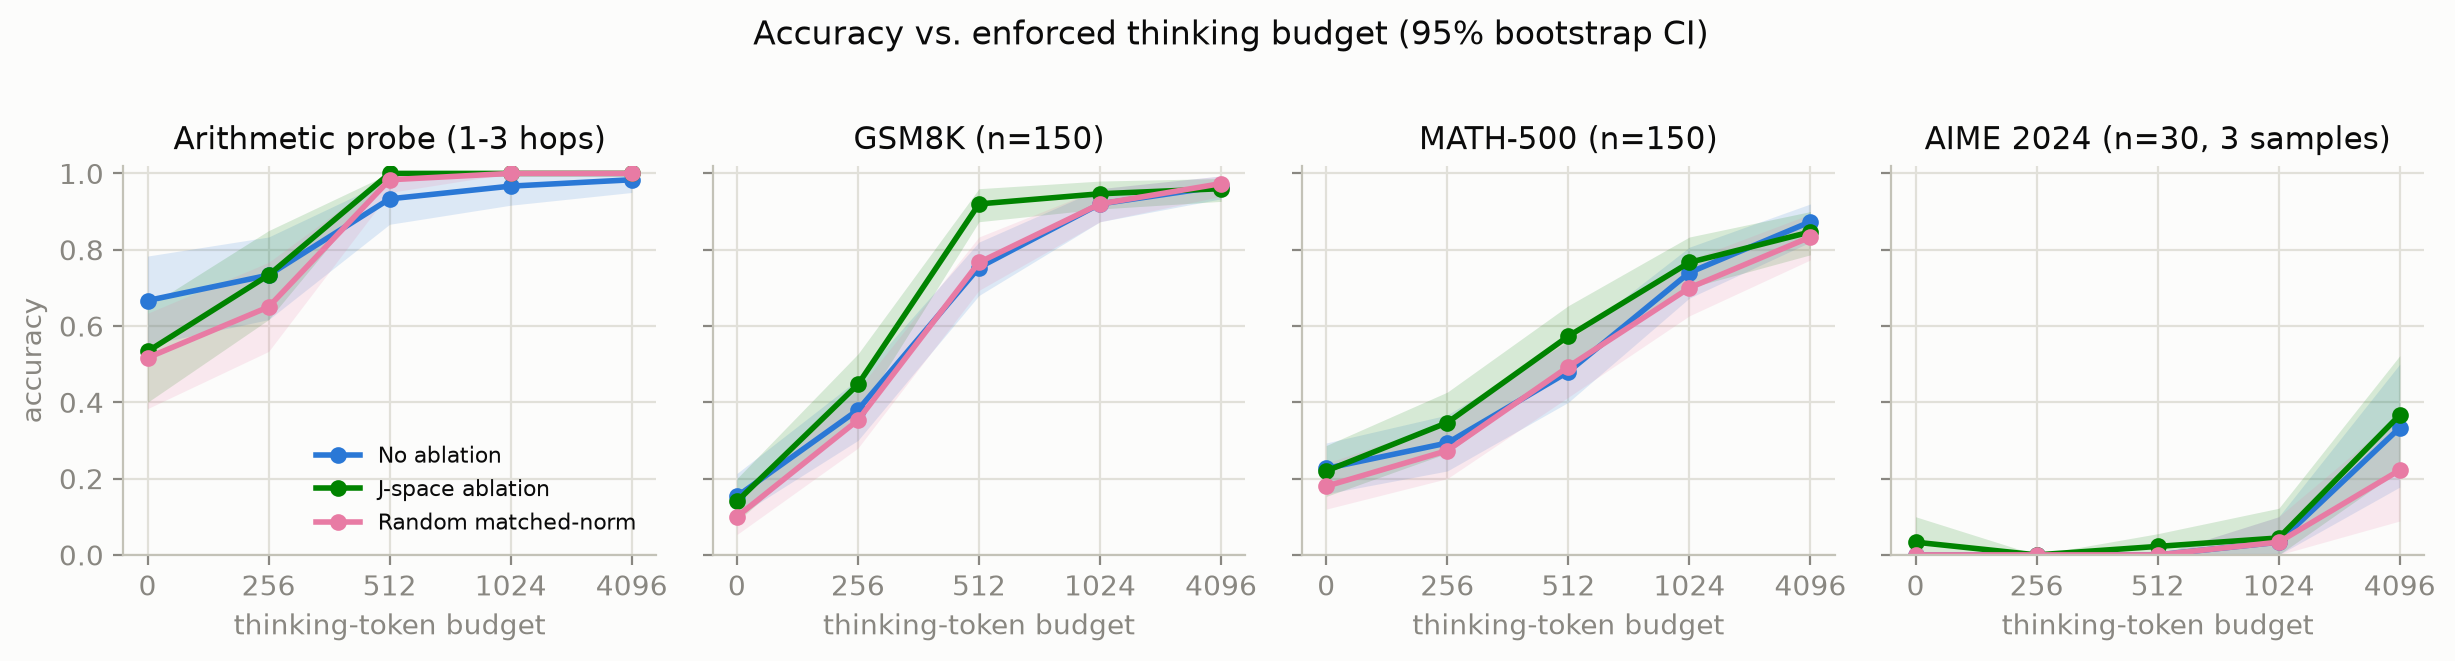
\includegraphics[width=\linewidth]{figs/fig1_dose_response.png}
  \caption{Accuracy versus enforced thinking budget by arm, with 95\%
    bootstrap confidence intervals.}
  \label{fig:dose}
\end{figure*}

\begin{table}[t]
  \setlength{\tabcolsep}{4pt}
  \centering
  \footnotesize
  \caption{GSM8K and MATH-500 accuracy by arm and thinking budget.}
  \label{tab:acc}
  \begin{tabular}{r ccc ccc}
    \toprule
    & \multicolumn{3}{c}{GSM8K} & \multicolumn{3}{c}{MATH-500} \\
    \cmidrule(lr){2-4} \cmidrule(lr){5-7}
    budget & ctrl & J-abl & rand & ctrl & J-abl & rand \\
    \midrule
    0    & .153 & .140 & .100 & .227 & .220 & .180 \\
    256  & .380 & \textbf{.447} & .353 & .293 & \textbf{.347} & .273 \\
    512  & .753 & \textbf{.920} & .767 & .480 & \textbf{.573} & .493 \\
    1024 & .920 & .947 & .920 & .740 & .767 & .700 \\
    4096 & .967 & .960 & .973 & .873 & .847 & .833 \\
    \bottomrule
  \end{tabular}
\end{table}

\paragraph{(a) No selective impairment at budget 0 (prediction 1 not
supported).} On GSM8K and MATH-500 the direct-answer baseline sits at the
floor calibration predicted, and J-ablation moves it by roughly one point
(McNemar $p = 0.80$ / $1.00$). On the arithmetic probe, whose baseline has
headroom (66.7\%), J-ablation does impair direct answering (53.3\%;
$p = 0.0078$) with a clean hop gradient --- 1-hop unaffected (100\%), 2-hop
75\% $\to$ 55\%, 3-hop 25\% $\to$ 5\% --- but the random arm lands in the
same place (51.7\%; 100/50/5\% by hops; J-space versus random $p = 1.0$).
The damage is multi-hop-specific but not J-space-specific.

\paragraph{(b) A J-space-specific accuracy gain at intermediate budgets.}
At budget 512 the J-ablated arm exceeds control by 16.7 points on GSM8K
(92.0\% vs 75.3\%; McNemar 27 vs 2, $p < 10^{-5}$) and 9.3 points on
MATH-500 (57.3\% vs 48.0\%; $p = 0.0043$), with the same sign at budget
256. Unlike the impairment in (a), this effect is specific to the J-space
directions: the random arm tracks control (76.7\% / 49.3\% at 512), and
paired J-space-versus-random tests give $p < 10^{-4}$ (GSM8K, 512),
$p = 0.024$ (GSM8K, 256), and $p = 0.017$ (MATH-500, 512).

\begin{figure*}[t]
  \centering
  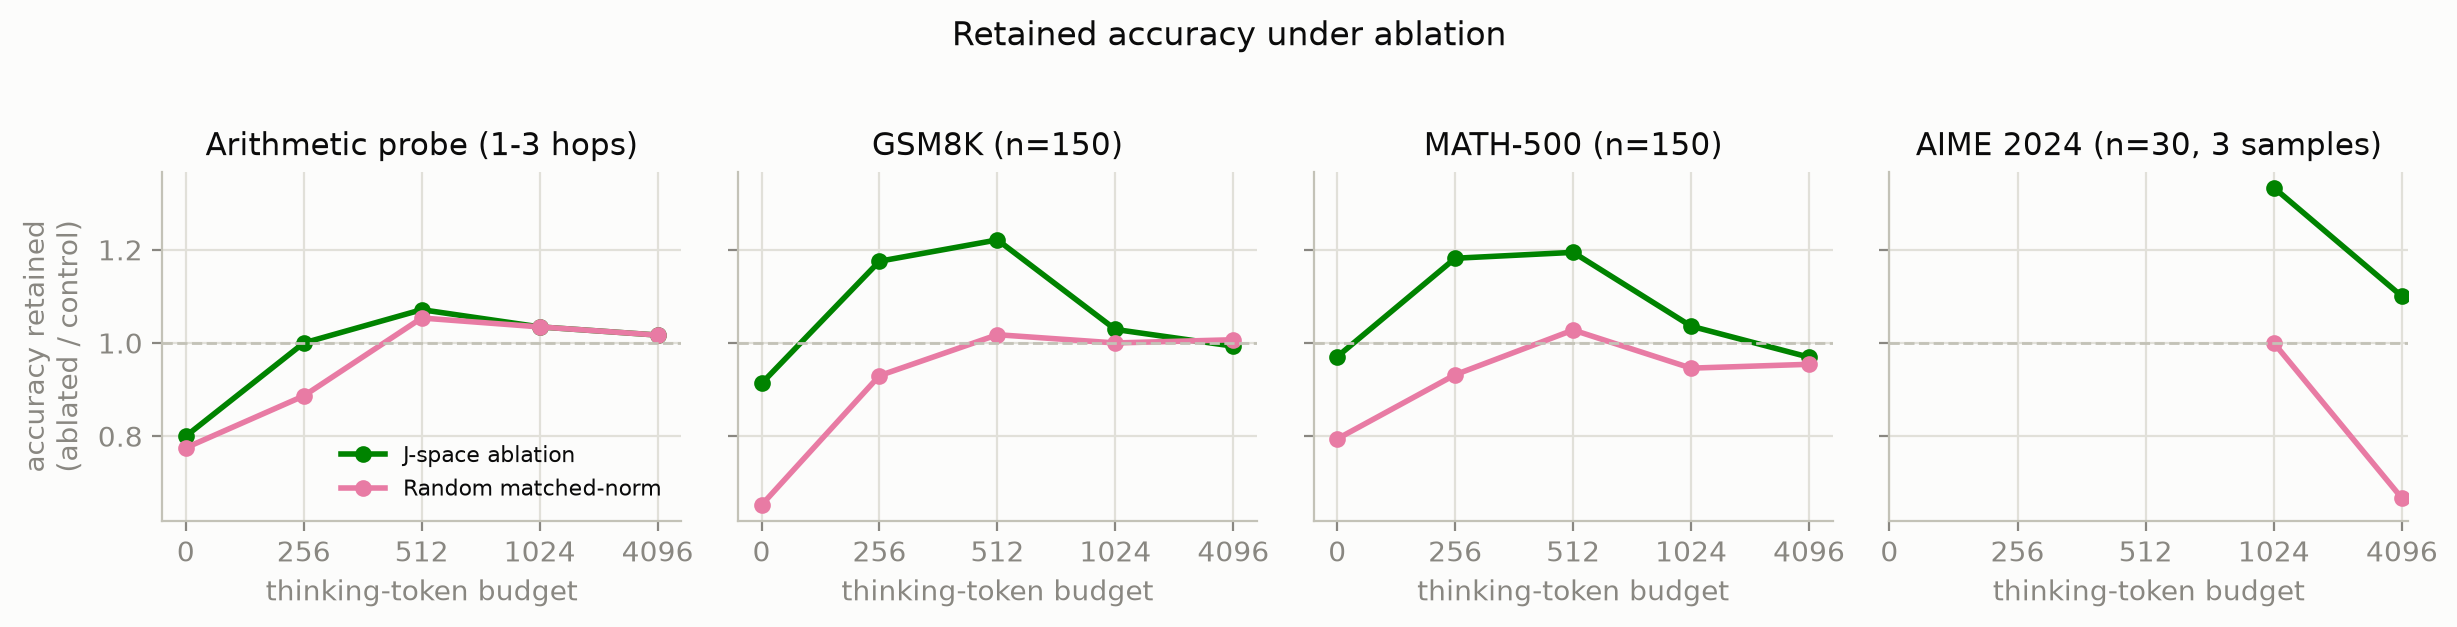
\includegraphics[width=\linewidth]{figs/fig4_rescue.png}
  \caption{Retained accuracy (ablated/control) by thinking budget. The
    random arm hovers near 1.0 while the J-ablated arm exceeds it at
    intermediate budgets; AIME points below budget 1024 are undefined
    because control accuracy is zero there.}
  \label{fig:rescue}
\end{figure*}

\paragraph{(c) The mechanism is shorter chain of thought (prediction 4
inverted).} At the effectively unconstrained 4{,}096 budget, J-ablated CoT
is consistently shorter: 1{,}202 versus 1{,}703 mean thinking tokens on
GSM8K (random: 1{,}642), 853 versus 1{,}049 on the arithmetic probe,
2{,}326 versus 2{,}657 on MATH-500 (length distributions:
\texttt{report/figs/fig5\_cot\_length.png}). The J-ablated arm is
correspondingly clipped less wherever clipping is common (GSM8K at 1024:
41\% versus 69\%), and the gain in (b) is concentrated exactly where
control chains are truncated mid-reasoning.

\paragraph{(d) Dose--response and convergence (prediction 2, weak form).}
Every arm rises steeply with budget and the arms converge by budgets
1024--4096 (GSM8K 96--97\%; MATH-500 83--87\%). CoT fully rescues the
arithmetic impairment --- the J-ablated arm reaches 100\% at budget 512
(control 93.3\%, random 98.3\%; all arms $\geq$96.7\% by 1024) --- but from
damage that was never J-space-specific.

\paragraph{(e) No difficulty interaction in the predicted direction
(prediction 3 not supported).} Within MATH-500 at budget 512 the
J-ablation \emph{advantage} appears at levels 1--4 ($+.10$, $+.17$, $+.10$,
$+.10$) and vanishes at level 5 (.23 both; per-level curves:
\texttt{report/figs/fig3\_difficulty.png}). AIME is floored below budget
4096 (0--4\%) and shows no significant arm differences at 4096 (control
33.3\%, J-ablated 36.7\%, random 22.2\%); 89--94\% of AIME chains still
clip at 4{,}096 tokens, so that condition largely measures truncation.

\section{Analysis of results}

Of the four pre-registered predictions, only the weak form of prediction 2
(rescue by CoT, with dose--response) survives. Prediction 1's selective
impairment appears only where the direct-answer baseline is off the floor,
and is matched by an equally large random perturbation; prediction 3's
difficulty interaction is absent; prediction 4 inverted. The one robustly
J-space-specific effect is opposite in direction to the hypothesis:
removing the top-$k$ J-lens directions makes written CoT shorter (median
paired length ratio 0.76) at equal or better accuracy. A post-hoc
transcript probe (\texttt{scripts/verify\_reflection.py}; 20 GSM8K problems
regenerated with full think-text, which the main run did not store) shows
the omitted content is disproportionately \emph{reflective}: J-ablated
chains carry fewer reflection markers per thinking token (6.7 vs 9.9 per
1{,}000; ``wait'' 1.9 vs 3.2, ``alternatively'' 1.6 vs 3.9, ``verify''
0.04 vs 0.25) --- roughly half the double-checking and re-derivation loops
per problem. This suggests the ablated directions in this band carry
self-monitoring or verbalization content rather than load-bearing
intermediate state; on this model the J-space--CoT relationship resembles
modulation of how much the model narrates, not an internal scratchpad for
which text substitutes.

Two qualifications: floor effects --- when externalization is genuinely
prevented, un-ablated Qwen3-4B scores 15--23\% on GSM8K/MATH-500 and 0\% on
AIME, leaving little internal reasoning to ablate, a caution against
extrapolating the paper's headline result to small thinking-tuned models
--- and alternative explanations: the wikitext-fitted community lens may
capture a shallower subspace than a paper-faithful lens, the random arm
matches removed norm per position but not its location in the residual
basis, and thinking-mode sampling adds variance. None of these plausibly
explains the intermediate-budget gain, which replicates across two datasets
with the random arm flat.

With more time or compute: a paper-faithful lens fit; $k$ and layer-band
sweeps with per-position delta-norm audits; clamping or patching individual
J-vectors to isolate the CoT-shortening direction; faithfulness checks on
the shortened chains; and replication on a larger model whose direct-answer
baseline is off the floor without a synthetic probe.

\end{document}
